\chapter{Practical Aspects}
\label{chap:practical}

\myLettrine{G}{iven} the previously described topology and theoretical model of the proposed solar inverter system in the last chapter, there is a need to implement this solution into a physical circuit in order to effectively determine the efficiency of this implementation.
This step is achieved by creating the design of a dedicated PCB that contains the \gls{H-bridge}, passive filtering circuitry and logic control sections, combined with the \gls{pid} controller and current measurements implemented at the software level.
The solution I am proposing in the following sections have been made with these energy targets in mind:

\begin{itemize}
    \item Input voltage ($V_{in}$) is $24V$ \gls{dc};
    \item Output voltage ($V_{out}$) is $24V$ \gls{ac};
    \item RMS current converted ($I_{RMS}$) is around $2.5A$;
\end{itemize}

thus converting the equivalent of $60W$.
These characteristics are only ideal, as there are no perfect components and energy losses are unavoidable, however for the scope of this thesis, this should be enough to demonstrate the efficiency of the chosen topology.

\section{Hardware Implementation}

The process of designing the electronic device is split into choosing the main components (microcontroller, switching elements, current measuring resistor, operational and instrumentation amplifiers, passive components specific to the filtering), drawing the schematic of the board, simulating the design and doing the PCB layout.
This has been done using KiCad, a free and open source CAD program that has more than enough features to aid in the development of the PCB in question.

\subsection{Component Selection}

Arguably the most important section of the whole circuit is the \gls{H-bridge}, which allows for the formation of the current sine wave present in any \gls{ac} signal.
In most common instances, the bridge is composed of 4 transistors, either MOSFETs or IGBTs, that act as electronically commanded switches to the inverter system. On this prototype, size and cost are a priority over efficiency and maximum power rating, as long as these components can achieve the proposed target.
For this, I have chosen 2 IFX007Ts, which are ICs containing a half-bridge and gate drivers, used primarily for motor control, but these can also be used in power conversion applications.
Since they can withstand up to $50A$ of current flowing through the drain and operate up to $40V$, these components satisfy the required targets.

Passive components chosen for the LCL filter are crucial in order to block residual high frequencies caused by the \gls{pwm} switching and any other external sources of noise.
Criteria for choosing these consist of low ESR values, which in turn would mean higher power conversion efficiency, tolerance values of the main characteristic of that component, maximum saturation current for the inductors and low ripple current for the capacitors.
Hybrid aluminum polymer capacitors exhibit such good values, and for inductors, specialized flexible transformer have been used, as the windings can be independently connected in serial and parallel configurations. This achieves different turn ratios, inductance and current-carrying capabilities.

\begin{figure}[!ht]
    \begin{center}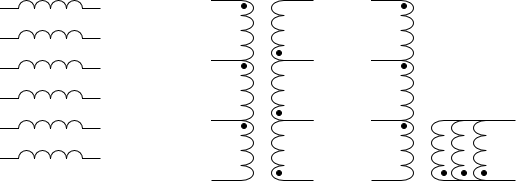
\includegraphics[width=\singlefigure]{\pics/schematics/transformerconfigs}\end{center}
    \caption{WE-FLEX transformer overview and example configurations}
    \label{fig:transf}
\end{figure}

The main take from \figref{fig:transf} is the following: the flexible transformer chosen can be thought of as 6 independent coils that can be connected in any way (as long as polarities are respected, market with a dot).
Knowing the base inductance per turn ($L_{base}$) is $12\mu H$ and the base current is $1.7A$, coils put in parallel multiply the base current rating, and windings put in series increase the inductance of the primary/secondary couple in accordance to this equation:
\be
\label{eq:Lwindings}
L_{res}=L_{base}\times N_{sw}^2
\ee
where $N_{sw}$ is the number of windings in series.
For the given examples, the middle configuration turns into a 1:1 ratio, $108\mu H$ transformer that can carry $1.7A$ of RMS current, and the right configuration is a 3:1 ratio transformer that has the same values on the primary as the former configuration, but the secondary can carry $5.1A$ with inductance $12\mu H$.

The feedback loop needs some way to have currents and voltages measured in order to calculate the next command to be given, thus a special current sense resistor is utilized in the circuitry.
This resistor has a low resistance value (usually under $1\Omega$), near 0\% tolerances and higher power ratings since they dissipate heat proportional to the current driven on the power traces, and it should not have its resistance drift with temperature changes.
Since we expect to deliver at least $2.5A$ RMS current through the PCB traces, and to have minimal voltage drop across the resistor's terminals, I've chosen the WSLP2512R0100FEA, which is a $10m\Omega$, $\pm 1\%$ SMD resistor that can withstand $3W$.
This is sufficient, as per Joule's first law:
\be
\label{eq:Joulefirstlaw}
P = I^2 \times R
\ee
it would result in a peak power dissipation of around $0.01\Omega \times (10A)^2 = 1W$, which is a third of the maximum power rating and a safe value to consistently maintain without damaging the component.
The voltage sensing terminals are then connected through \gls{Kelvin connection} to operational amplifiers and instrumentation amplifiers, like the MCP6001 and the AD8148 series respectively, used for amplifying the signal's gain and reject common-mode signals.
Current can't be directly measured, however the voltage drop on the shunt can be quantified, and since it is defined to be small in order to minimize losses, gain amplification needs to be done. To calculate the source current, we can use Ohm's law:
\be
\label{eq:Ohmslaw}
V = I \times R
\ee
where the voltage is measured and resistance is already known.

All of these functions are tied to the microcontroller, that converts the values measured of the analog signals using the \gls{adc}s into numeric values, and these values are used as reference and system output in order to recalculate the \gls{pwm} duty cycles which modulates the carrier signal through the \gls{gpio}, or in this case, the converted \gls{ac} power source.